\documentclass[aspectratio=169,
  hyperref={colorlinks=true,linkcolor=black,citecolor=blue,urlcolor=blue}
]{beamer}
\usepackage{graphicx} % Allows including images
\usepackage{booktabs} % Allows the use of \toprule, \midrule and \bottomrule in tables
\usepackage{tikz,pgfplots}
\usepackage{fontspec}
\usepackage[absolute,overlay]{textpos}

\usetikzlibrary{shapes, snakes, arrows}

\setlength{\TPHorizModule}{10mm}
\setlength{\TPVertModule}{\TPHorizModule}
\textblockorigin{1mm}{1mm} % start everything near the top-left corner
\setlength{\parindent}{0pt}
%\usefonttheme{serif}
\setbeamerfont{footnote}{size=\tiny}
\setsansfont{Bookerly}


\beamertemplatetransparentcovereddynamic
\beamertemplatesolidbuttons
\beamertemplateroundedblocks
\definecolor{azul}{RGB}{1,80,159}
\definecolor{azulclaro}{RGB}{230,230,255}
\setbeamercolor{titlelike}{fg=azul}
\setbeamercolor{block title}{fg=white}
\setbeamercolor{block title}{bg=azul}
\setbeamercolor{block body}{bg=azulclaro}

%%%%%%%%%%%%%%%%%%%%%%%%%%%%%%%%%%%%%%%%%%%%%%%%%%%%%%%%%%%%%%%%%%%%%%%%%%%%%%%%%%%%%%%%%%%%%%%%%%%%%%%%%%%%%%%%%%%%%

\newcommand{\incertarlogo}{\begin{textblock}{3}(10.5,0)
    \centering 
    \definecolor{colora}{rgb}{0.66,0.69,0.2} 
    \definecolor{colorb}{RGB}{103,99,74} 
    \definecolor{colorc}{RGB}{7,78,64} 
    \definecolor{colord}{RGB}{2,151,93} 
    \definecolor{colore}{RGB}{0,59,88} 
    \definecolor{colorf}{RGB}{0,128,189} 
    \definecolor{colorg}{RGB}{212,22,47} 
    \definecolor{colorh}{RGB}{226,112,42} 
    \definecolor{colori}{RGB}{237,173,24} 
    \definecolor{colorj}{RGB}{103,20,46} 
    \begin{tikzpicture}[x=0.1mm,y=0.1mm]          
        \draw[colorc, fill] (30,-30) -- +(0,30) -- +(10,30) -- +(10,0) -- cycle;     
        \draw[colorb, fill] (10,-30) -- +(30,0) -- +(20,-10) -- +(0,-10) -- cycle;         
        \draw[colora, fill] (0,0) -- +(0,-30) -- +(10,-40) -- +(10,10) -- cycle;             
        \draw[colord, fill] (30,0) -- +(10,10) -- +(30,10) -- +(20,0) -- cycle;     
        \draw[colorf, fill] (53,0) -- +(0,-40) -- +(10,-30) -- +(10,0) -- cycle;     
        \draw[colore, fill] (53,0) -- +(10,10) -- +(30,10) -- +(20,0) -- cycle;     
        \draw[colori, fill] (107,-12) -- +(-20,0) -- +(-20,-10) -- +(0,-10) -- cycle ;     
        \draw[colorh, fill] (107,0) -- +(10,0) -- +(10,-12) -- +(0,-22) -- cycle;     
        \draw[colorg, fill] (77,0) -- +(10,10) -- +(30,10) -- +(40,0) -- cycle;     
        \draw[colorj, fill] (87,-12) -- +(-10,-10) -- +(-10,-28) -- +(0,-18);         
    \end{tikzpicture} \end{textblock} 
    }

%%%%%%%%%%%%%%%%%%%%%%%%%%%%%%%%%%%%%%%%%%%%%%%%%%%%%%%%%%%%%%%%%%%%%%%%%%%%%%%%%%%%%%%%%%%%%%%%%%%%%%%%%%%%%%%%%%%%%
\definecolor{pagenum}{RGB}{173, 173, 224}
\newcommand{\mframe}[1]{
    \frame{
        \begin{textblock}{3}(0, 8.6)
            \color{pagenum}\tiny\insertframenumber\,/\,\inserttotalframenumber
        \end{textblock}

        #1}
}
%%%%%%%%%%%%%%%%%%%%%%%%%%%%%%%%%%%%%%%%%%%%%%%%%%%%%%%%%%%%%%%%%%%%%%%%%%%%%%%%%%%%%%%%%%%%%%%%%%%%%%%%%%%%%%%%%%%%%%%
\usepackage{listings}
\lstset{frameround=fttt,language=Python, keywordstyle=\color{blue!30!green}, tabsize=4, commentstyle=\color{orange},
    basicstyle=\ttfamily, numbers=left,numberstyle=\tiny}


\usepackage{mathtools}
\mathtoolsset{showonlyrefs}

\usepackage{graphicx}
\usepackage{subfigure}
\usepackage{ctex}
\usepackage{multirow}
\usepackage{makecell}
\usepackage{pgfplots}
\usepackage{tikz}
\usetikzlibrary{positioning, arrows.meta}
\usepgfplotslibrary{groupplots}    % 用于显示多图
\usepackage[backend=biber,style=authoryear]{biblatex}
\addbibresource{ref.bib}
\setbeamertemplate{bibliography item}{}
\linespread{1.2}

\newcommand\paper[4]{\definecolor{black}{RGB}{0.66,0.69,0.2}\begin{frame}
  \centering \Large \color{azul}{#1}\\
  \vspace{20pt}
  \large \color{black}{#2}\\
  \vspace{10pt}
  \normalsize \color{black}{#3}\\
  \vspace{10pt}
\end{frame}}

\newcommand\linetext[1]{
  \resizebox{\textwidth}{!}{#1}
}

\graphicspath{{./imgs/}}
\def\bibfont{\scriptsize}
\def\titletext{Introduction to PLM}

\begin{document}
\begin{frame}
  \centering \Huge \color{azul}{\titletext}
  \vspace{20pt}
  \begin{figure}
    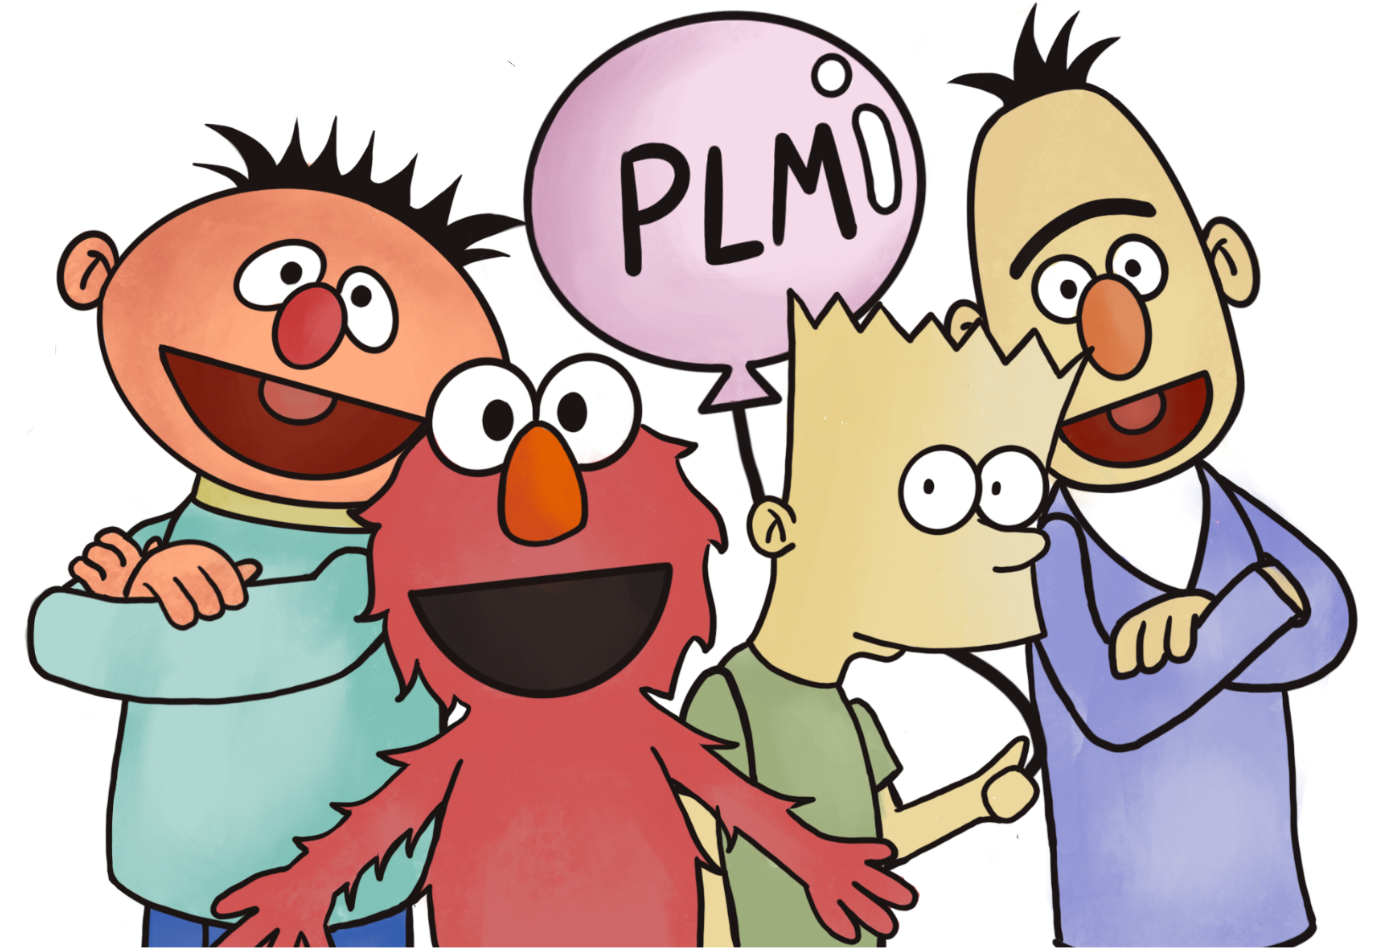
\includegraphics[height=\textheight/2]{1.png}
  \end{figure}
\end{frame}
\mframe{
  \frametitle{Introduction to PLM}
  PLM: Pre-trained Language Model
  \begin{itemize}
    \item Transformer Layer 结构
    \item Self-Attention 过程
    \item PLM 的结构和预训练目标
  \end{itemize}
}
\mframe{\frametitle[LM as RL]{Think Language Modeling as Representation Learning}
  \begin{itemize}
    \item 表征学习是深度学习的主要方法,深度神经网络的自动特征提取器以表征向量的形式建模样本特征,以用于实际任务
    \item 自 \Textcite{Bengio2003} 将前馈神经网络引入自然语言处理以来,表征学习就是语言建模的主要方法
  \end{itemize}
  对于长度为 $L$ 的自然语言语句 $\mathbf{s}=\{x_1, x_2, ..., x_L\}$, 其中 $x_i$ 是自然语言 token,表征计算即如下的过程:

$$[\mathbf{h}_1, \mathbf{h}_2, ..., \mathbf{h}_L] = \text{Encoder}(\mathbf{x}_1, \mathbf{x}_2, ..., \mathbf{x}_L)$$

其中 $\mathbf{x}_i$ 是 token $x_i$ 的嵌入向量,$\mathbf{h}_i$ 是 $x_i$ 的表征,$\text{Encoder}$ 是一个神经网络编码器。
}
\mframe{\frametitle{Neural Encoder}
  神经语言(序列)编码器根据每层中的基本编码单元可以分为三种:
  \begin{itemize}
    \item Convolutional Language Encoder
    \item Recurrent Language Encoder
    \item Self-Attention Language Encoder: 
    可以简述为:在进行序列表征学习(序列建模)时,让模型自动选择基于该序列 (Self) 的哪些部分进行计算,即:
    $\mathbf{h}_i=\sum_{j=1}^L\alpha_{ij}\mathbf{x}_j$, $\alpha_{ij}$ 即注意力参数
  \end{itemize}
  \begin{figure}
    \subfigure[CNN Encoder]{
      \begin{minipage}[b]{0.3\linewidth}
        \centering
        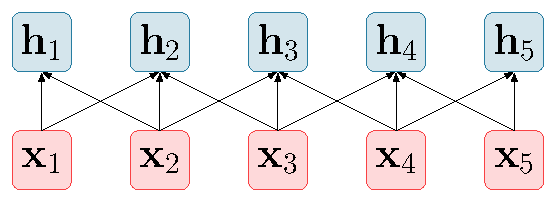
\includegraphics[width=\textwidth]{cnn.pdf}
      \end{minipage}
    }
    \subfigure[RNN Encoder]{
      \begin{minipage}[b]{0.3\linewidth}
        \centering
        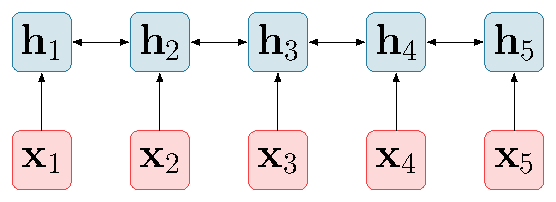
\includegraphics[width=\textwidth]{rnn.pdf}
      \end{minipage}
    }
    \subfigure[Self-Attn Encoder]{
      \begin{minipage}[b]{0.3\linewidth}
        \centering
        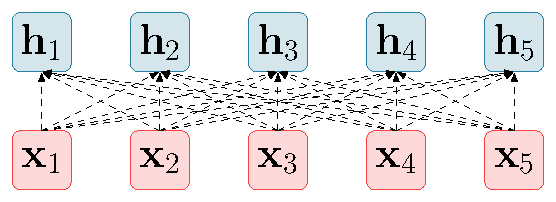
\includegraphics[width=\textwidth]{attn.pdf}
      \end{minipage}
    }
  \end{figure}
}
\mframe{\frametitle{一种 Self-Attn Encoder: Transformer Layer}\label{TransformerLayer}
  \begin{columns}
    \begin{column}{0.7\linewidth}
      \Textcite{Vaswani2017a} 在 \citetitle{Vaswani2017a} 中提出了一种完全基于注意机制的
      语言模型,并在机器翻译,语法解析等任务上达到了 sota.\\
      其模型的重要结构:Transformer Layer 成为后续
      深度语言模型的基础\\
      
      Transformer Layer 包括两个子层:
      \begin{itemize}
        \item Self-Attention sub-layer
        \item Feed-Forward sub-layer
      \end{itemize}
      每个子层还使用了 Residual Connection \Parencite{he2016} 和 Layer Normalization \Parencite{ba2016}.\\
      
      下面分别介绍这些结构
    \end{column}
    \begin{column}{0.3\linewidth}
      \begin{figure}
        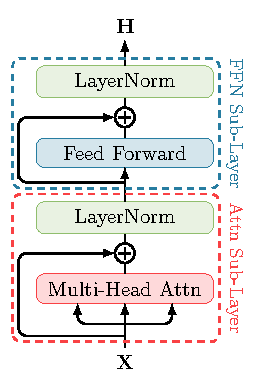
\includegraphics[width=0.9\textwidth]{transformer-layer.pdf}
        \caption{Transformer Layer}
      \end{figure}
    \end{column}
  \end{columns}
}
\mframe{\frametitle{Attention sub-layer}
  Attention sub-layer 是模型的核心,即:如何计算注意力分数($\alpha_{ij}$).\\
  Transformer 使用 Query-Key-Valye(QKV) 模型实现这部分计算\\
  下面以如下的顺序介绍 transformer 中的 QKV 计算过程:
  \begin{itemize}
    \item 首先介绍 Scaled dot-product attention 的计算过程(基本的 QKV 计算过程)
    \item 然后介绍其计算形式上的合理性
    \item 最后介绍 transformer 的 attention sublayer 
    中使用的 multi-head attention 的计算过程(Transformer 使用的一个 trick)
  \end{itemize}
}

\mframe{\frametitle{Scaled dot-product attention}
  \begin{itemize}
    \item 首先计算 $\mathbf{Q}, \mathbf{K}, \mathbf{V}$:
    $$\mathbf{Q}, \mathbf{K}, \mathbf{V} = \mathbf{X}\mathbf{W}^Q,
    \mathbf{X}\mathbf{W}^K, \mathbf{X}\mathbf{W}^V$$
    其中 $\mathbf{X} = \text{concat}(\mathbf{x}_1, \mathbf{x}_2, ..., \mathbf{x}_L)$ 
    是输入文本嵌入向量的拼接,$\mathbf{W}^Q, \mathbf{W}^K, \mathbf{W}^V$ 是投影矩阵,也是模型参数
    \item 然后通过以下过程计算表征:
    $$\mathbf{H}=\text{Attn}(\mathbf{Q}, \mathbf{K}, \mathbf{V}) =
    \text{softmax}(\frac{\mathbf{QK}^\top}{\sqrt{d_k}})\mathbf{V}$$
    其中 $d_k$ 是模型维度,$\mathbf{H}\in\mathbb{R}^{L\times d_k}$
    是输出表征的拼接矩阵,即:$\mathbf{h}_i = \mathbf{H}[i, :], \forall i\in[1, L]$
  \end{itemize}
}
\newcounter{romanc}
\stepcounter{romanc}
\mframe{
  \frametitle{为什么有效? \Roman{romanc}}
  明确两个观点:
  \begin{itemize}
    \item self-attention 过程 $\mathbf{h}_i=\sum_{j=1}^L\alpha_{ij}\mathbf{x}_j$
    即对输入序列某些部分的选择,自然的,QKV 计算也是在模拟该过程
    \item 向量内积相当于相似度计算
  \end{itemize}
  然后考虑 self-attention 计算的一个简化版:
  \[\text{Attn}(\mathbf{X}) = \text{softmax}(\mathbf{XX}^\top)\mathbf{X}\]
  其中 $\mathbf{X} = [\mathbf{x}_1; \mathbf{x}_2; ...; \mathbf{x}_L]$, $\mathbf{x}_i$ 
  是 $d_k$ 维行向量,代表 token $i$ 的嵌入向量。
}
\stepcounter{romanc}
\mframe{\frametitle{为什么有效? \Roman{romanc} ---- {$\text{Attn}(\mathbf{X})=\text{softmax}(\mathbf{XX}^\top)\mathbf{X}$}}
  分析其行为:
  \begin{columns}
    \begin{column}{0.5\linewidth}
        \begin{itemize}
          \item $$\begin{aligned}
          \mathbf{XX}^\top &= \left[\begin{matrix}
              \mathbf{x}_1\\
              \mathbf{x}_2\\
              \vdots\\
              \mathbf{x}_L
          \end{matrix}\right]\cdot
          [\mathbf{x}_1^\top, \mathbf{x}_2^\top, \cdots, \mathbf{x}_L^\top]\\
          &=\left[\begin{matrix}
              \mathbf{x}_1\mathbf{x}_1^\top &\mathbf{x}_1\mathbf{x}_2^\top &\cdots &\mathbf{x}_1\mathbf{x}_L^\top\\
              \mathbf{x}_2\mathbf{x}_1^\top &\mathbf{x}_2\mathbf{x}_2^\top &\cdots &\mathbf{x}_2\mathbf{x}_L^\top\\
              \vdots &\vdots &\ddots &\vdots\\
              \mathbf{x}_L\mathbf{x}_1^\top &\mathbf{x}_L\mathbf{x}_2^\top &\cdots &\mathbf{x}_L\mathbf{x}_L^\top
          \end{matrix}\right]\\
          &\in\mathbb{R}^{L\times L}
          \end{aligned}$$    
        \end{itemize}
    \end{column}
    \begin{column}{0.5\linewidth}
      显然, $\mathbf{x}_i\cdot\mathbf{x}_j^\top$ 的结果表征的是向量 $\mathbf{x}_i$ 和 $\mathbf{x}_j$ 之间的相似度。\\
      于是 $(\mathbf{XX}^\top)_{ij}$ 具备了 $\alpha_{ij}$ 的作用:描述了第 $i,j$ 个 token 之间的关系
    \end{column}
  \end{columns}

}
\stepcounter{romanc}
\mframe{
  \frametitle{为什么有效? \Roman{romanc} ---- {$\text{Attn}(\mathbf{X})=\text{softmax}(\mathbf{XX}^\top)\mathbf{X}$}}
  \begin{itemize}
    \item Softmax 函数可以简单理解为一种归一化手段,它将上述向量内积的结果归一化到 $(0, 1)$ 的范围内,且同一行中所有值的和为 $1$. 
    这样,上述过程中 $\text{softmax}(\mathbf{XX}^\top)$ 的结果可以认为是一个归一化的加权矩阵
    \item 最后一步的意义是显然的:根据前面计算的加权矩阵为输入序列的嵌入计算加权和,作为输出表征,
    即 $\mathbf{h}_i = \sum_{j=1}^L\alpha_{ij}\mathbf{x}_j$ 的过程.
  \end{itemize}
  下面是这个过程的一个图示
}
\stepcounter{romanc}
\mframe{
  \frametitle{为什么有效? \Roman{romanc} ---- {$\text{Attn}(\mathbf{X})=\text{softmax}(\mathbf{XX}^\top)\mathbf{X}$}}
  \begin{figure}
    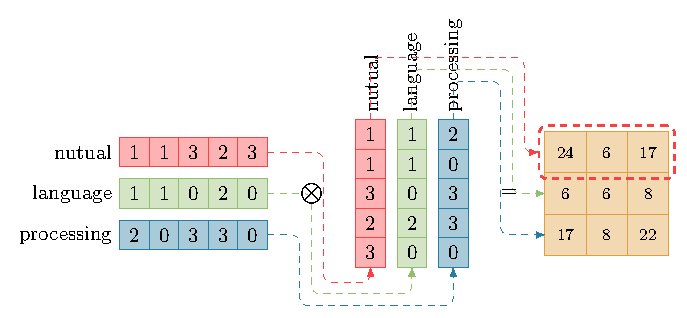
\includegraphics[width=\textwidth]{scaled-dot-product-attn.pdf}
  \end{figure}
}
\stepcounter{romanc}
\mframe{
  \frametitle{为什么有效? \Roman{romanc} ---- {$\text{Attn}(\mathbf{X})=\text{softmax}(\mathbf{XX}^\top)\mathbf{X}$}}
  \begin{figure}
    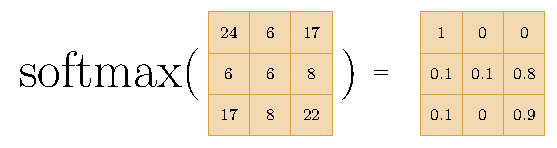
\includegraphics[width=\textwidth]{scaled-dot-product-attn1.pdf}
  \end{figure}
  \footnotetext{$\text{softmax}(\mathbf{x})=\frac{\exp(\mathbf{x})}{\sum\exp(\mathbf{x})}$}
}
\stepcounter{romanc}
\mframe{
  \frametitle{为什么有效? \Roman{romanc} ---- {$\text{Attn}(\mathbf{X})=\text{softmax}(\mathbf{XX}^\top)\mathbf{X}$}}
  \begin{figure}
    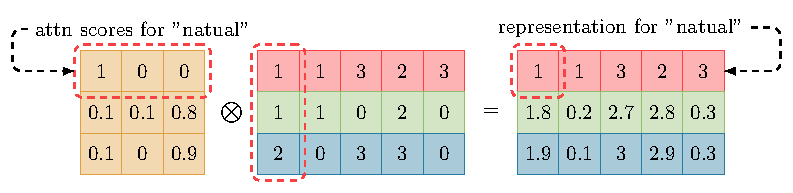
\includegraphics[width=\textwidth]{scaled-dot-product-attn2.pdf}
  \end{figure}
}
\stepcounter{romanc}
\mframe{\frametitle{为什么有效? \Roman{romanc} ---- 回到 QKV}
  与 QKV 的计算过程相比,上面讨论的简化版本主要有以下区别:
  \begin{itemize}
    \item 文本序列的输入嵌入首先经过线性投影才参与计算,而不是直接计算
    \item 注意力分数在归一化之前要先经过一个缩放系数 $\sqrt{d_k}$
  \end{itemize}
  \vspace{0.5cm}
  \[\begin{cases}
    \text{softmax}(\frac{\mathbf{QK}^\top}{\sqrt{d_k}})\mathbf{V},
    where: \mathbf{Q}, \mathbf{K}, \mathbf{V} = \mathbf{X}\mathbf{W}^Q, \mathbf{X}\mathbf{W}^K, \mathbf{X}\mathbf{W}^V\\
    \text{softmax}(\mathbf{XX}^\top)\mathbf{X}
  \end{cases}\]
  \vspace{0.5cm}
  下面解释其原因
}
\stepcounter{romanc}
\mframe{
  \frametitle{为什么有效? \Roman{romanc}}
  \begin{itemize}
    \setlength{\itemsep}{.3cm}
    \item $\mathbf{W}^Q, \mathbf{W}^K, \mathbf{W}^V$ 三个矩阵都是与输入相乘而起作用,
    其本质是对输入表征进行线性变换,主要的信息仍然是 $\mathbf{X}$,其意义在于:
    \begin{itemize}
      \setlength{\itemsep}{.1cm}
      \item 提升模型的拟合能力。三个线性变换相当于线性层,属于神经网络的一种
      \item 如果不使用这三个线性变换,$\mathbf{XX}^\top$ 的结果中,$\mathbf{XX}^\top_{ii}$ 的值,
      即每个 token 对自己的注意力将会大大超过对其他 token 的注意力,经过 softmax 之后其他 token 的
      attention score 会被严重挤压
    \end{itemize}
    \item 缩放系数 $\sqrt{d_k}$ 对矩阵的内积进行缩放:
    \begin{itemize}
      \item 如果不进行缩放,在 $d_k$ 即向量维度很大时向量之间的内积也会很大,这样经过 softmax
      之后的梯度会非常小\footnote{
        例如对于均值为 $0$, 方差为 $1$ 的 $d_k$ 维向量 $\mathbf{q}, \mathbf{k}$, 
        他们内积结果 $\mathbf{q}\cdot\mathbf{k}^\top$ 的均值为 $0$, 方差为 $d_k$.
        当 $d_k$ 很大时, 意味着分布 $\mathbf{q}\cdot\mathbf{k}^\top$ 的值集中在绝对值大的区域,
        即 $\text{softmax}(\mathbf{q}\cdot\mathbf{k}^\top)$ 的大部分值之间的梯度很小。
        因此需要以 $\sqrt{k}$ 进行缩放,使内积结果的方差为 $1$
      }
    \end{itemize}
  \end{itemize}
  如上就是 self-attention 中 scaled dot-product attention 的主要内容,实际上 transformer
  模型中使用的是它的简单复合:Multi-Head Attention
}
\mframe{
  \frametitle{Multi-Head Attention}

  Multi-Head Attention 具体地说,就是将 $\mathbf{Q}, \mathbf{K}, \mathbf{V}$ 三个矩阵进一步投影到 $h$ 个子空间,
  然后进行 self-attention 计算:
  $$\text{head}_i = \text{Attn}(\mathbf{QW}_i^Q, \mathbf{KW}_i^K, \mathbf{VW}_i^V)$$

  其中 $i\in[1,h]$, $\mathbf{W}_i^Q, \mathbf{W}_i^K\in\mathbb{R}^{d_\text{model}\times d_k}$,
  $\mathbf{W}_i^V\in\mathbb{R}^{d_\text{model}\times d_v}$

  $d_k$, $d_v$ 是一个比 $d_\text{model}$ 小的值,在 \citetitle{Vaswani2017a} 中, 
  作者取 $h=8, d_k=d_v=d_\text{model}/h$
}
\mframe{
  \frametitle{Multi-Head Attention}
  在 $h$ 个子空间进行 self-attention 计算将对每个词获得 $h$ 个 $d_v$ 维度的表征,
  Multi-Head Attention 将它们拼接起来并投影回 $d_\text{model}$ 维度。

  $$\text{MultiHead}(\mathbf{Q}, \mathbf{K}, \mathbf{V}) = \text{concat}(\text{head}_1, ..., \text{head}_h)\mathbf{W}_O$$

  其中 $\mathbf{W}_O\in\mathbb{R}^{hd_v\times d_\text{model}}$ 是投影矩阵
}
\mframe{
  \frametitle{Multi-Head Attention}
  关于为什么要做 Multi-Head Attention, \Citeauthor{Vaswani2017a} 称:\\
  在 Scaled dot-product attention 中,输入表征直接被投影到 $d_k$ 维度的 Query, Key, Value 向量,
  然后进行 self-attention 的加权平均过程。
  这个过程抑制了模型从\textbf{多个方面}提取文本序列的特征\\
  \vspace{0.2cm}
  实际上作者的代码里是将 $d_k$ 维度的 Query, Key, Value 切分成 $h$ 份,
  分别执行 self-attention 计算后拼接并投影\\
  \vspace{0.2cm}
  猜测这只是实践中发现效果更好的一个 trick\\
  \vspace{0.2cm}
  至此就是 Transformer 模型中关于 self-attention sublayer 的全部内容\footnote{
    BERT 中推荐阅读的 transformer 模型解释: http://nlp.seas.harvard.edu/2018/04/03/attention.html
  }
}
\mframe{
  \frametitle{Feed-Forward Layer}
  Feed-Forward sublayer 是一个全连接层,由两个线性层和 ReLU 激活函数组成,
  它对所有 token 的表征分别进行同等的变换:

  $$\text{FFN}(\mathbf{x}) = \text{ReLU}(\mathbf{xW}_1 + \mathbf{b}_1)\mathbf{W}_2 + \mathbf{b}_2$$

  虽然 self-attention 是 transformer 成功的关键,但是 FFN 层的参数量实际上是 self-attention 层的两倍,
  以 Transformer 模型为例,\Citeauthor{Vaswani2017a} 使用的参数是 $d_\text{model}=512$, 
  而 FFN 层的隐藏层维度是 $d_{ff}=2048$。\\
  一些工作认为预训练的 transformer 模型中 FFN 层存储着与下游任务相关的信息, 
  而 self-attention 层中存储的则是文本之间如何进行有效交互的模式 (\Cites{Geva2021}{He2022}).
}
\mframe{
  \frametitle{Residual Connection and Layer Normalization}
  Residual Connection \Parencite{he2016} 和 Layer Normalization \Parencite{ba2016}
  都是为解决深度模型训练困难的实践性问题提出的,并无理论解释。
  \begin{itemize}
    \item  对于 Residual Connection,自提出(\citetitle{he2016})以来,就一直是深度模型必备的部分,
  它主要解决了在过深的模型中训练时梯度(信息)消失的问题。
    \item 对于 Layer Normalization,它是针对 Batch Normalization \Parencite{ioffe2015}
    难以应用在 RNN 中的问题提出的。Normalization 操作简而言之就是将神经网络中每层的输出(神经元激活分数)的分布
    恢复为均值为 $0$, 方差为 $1$ 的正态分布,解决 Interval Covariate Shift 问题。
  \end{itemize}
}
\mframe{
  \frametitle{总结 Self-Attention Layer}
  \begin{itemize}
    \item  总的计算过程为:
  \[\begin{aligned}
    \mathbf{H}_\text{attn} &= \text{LayerNorm}(\text{MultiHead}(\mathbf{X}) + \mathbf{X})\\
    \mathbf{H}_\text{ffn} &= \text{LayerNorm}(\text{FFN}(\mathbf{H}_\text{attn}) + \mathbf{H}_\text{attn})
  \end{aligned}\]
  $\mathbf{H}_\text{ffn}$ 即最终的输出表征。
    \item Why Self-Attention?\\
    可以从以下三个方面考虑 self-attention 替代 CNN 和 RNN 的益处 \Parencite{Vaswani2017a}:\\
    \vspace{0.3cm}
    \begin{tabular}{lccc}
      \hline
      LayerType &每层的计算复杂度 &需要串行计算的操作 &最大路径长度\\
      \hline
      Self-Attention &$O(n^2\cdot d)$ &$O(1)$ &$O(1)$\\
      RNN &$O(n\cdot d^2)$ &$O(n)$ &$O(n)$\\
      CNN &$O(k\cdot n\cdot d^2)$ &$O(1)$ &$O(\log_k(n))$\\
      \hline
    \end{tabular}
  \end{itemize}
}
\mframe{
  \frametitle{PLM}
  较早的预训练语言模型如 word2vec \Parencite{mikolov2013}, GloVe \Parencite{erhan2010}
  等词嵌入模型在语料库上将词映射到静态的向量,这些向量相当于\textbf{上下文无关}的词表征,无法表示词的多义性。\\
  \Textcite{peters2018} 提出的 ELMo 使用双向 LSTM 网络计算上下文表征。ELMo 在使用时仅作为文本特征提取器嵌入到下游任务模型。
  随着 transformer 模型和预训练-微调模式的出现,仅作为特征提取器的预训练模型很快消失,ELMo 基本成为这类预训练模型的绝唱。
}
\mframe{
  \frametitle{PLM 结构}
  在 transformer 时代,PLM 根据模型架构可以分为三种:
  \begin{itemize}
    \item Encoder based(e.g., BERT\Parencite{devlin2019}, RoBERTa\Parencite{Liu2019}, XLNet\Parencite{Yang2019}.)
    \item Decoder based(e.g., GPT-1\Parencite{Radford2018}, GPT-2\Parencite{Radford2019}, GPT-3\Parencite{Brown2020}.)
    \item Encoder-Decoder based(e.g., BART\Parencite{lewis2019}, MASS\Parencite{Song2019}.)
  \end{itemize}
  模型的结构可以理解为用于计算表征的函数形式,对于参数化的深度模型 $f(\cdot; \Theta)$ 而言,就是 $f$ 的形式\\
  除形式外,还需要合适参数 $\Theta$ 才能实现好的表征计算,参数在训练中优化的方向则由\textbf{训练目标}决定
}
\mframe{
  \frametitle{预训练目标}
  语言模型预训练指在无标注的语料库上训练模型参数,通常使用自监督模式。\\
  \textbf{预训练目标}这一概念所涵盖的范围包括\textbf{自监督的具体方法}和\textbf{损失函数}
  在 PLM 中主要有三种预训练目标,基本与前述三种模型结构相对应:
  \begin{itemize}
    \item Autoencoding Modeling $\Rightarrow$ Encoder Model
    \item Autoregressive Modeling $\Rightarrow$ Decoder Model
    \item Sequence2Sequence Modeling $\Rightarrow$ Encoder-Decoder Model
  \end{itemize}
}
\mframe{
  \frametitle{Autoencoding Modeling}
  Autoencoding 的自监督是通过降噪受损的文本实现的,具体来说,就是首先向原始文本中注入噪音,
  将其变为受损的文本,然后训练模型恢复受损的部分,训练的损失仅根据受损部分的文本计算,损失函数可以表示为:
  \[\mathcal{L}_\text{AE}(\hat{\mathbf{X}})=\sum_{x_i\in m(\mathbf{X})}\log P(x_i|\mathbf{X}\backslash m(\mathbf{X}))\]
  其中 $\mathbf{X}$ 是输入序列,$\hat{\mathbf{X}}$ 是原始文本序列经过噪音函数后的文本序列
  $\hat{\mathbf{X}} = f_\text{noise}(\mathbf{X})$,$m(\mathbf{X})$ 是输入序列中受损的部分。
}
\mframe{
  \frametitle{Autoregressive Modeling}
  Autoregressive Modeling 有时也称 Standard Language Modeling(SLM),
  GPT 系列模型就是 Autoregressive 模型。Autoregressive 模型是一种单向生成模型,
  它的自监督模式是通过\textbf{上文信息}训练模型预测生成下一个词,训练损失为:
  \[\mathcal{L}_\text{AR}(\mathbf{X}) = \sum_{i=1}^{|\mathbf{X}|}\log P(x_i|x_1, x_2, ..., x_{i-1})\]
}
\mframe{
  \frametitle{Sequence-2-Sequence Modeling}
  Seq2Seq 的自监督过程是 Autoencoding 和 Autoregressive 过程的结合:
  首先向输入文本加入噪音,然后训练模型基于受损的文本使用编码器和解码器恢复出原始文本,
  其训练损失是恢复文本与原始文本之间的负对数似然:
  \[\mathcal{L}_{SS} = \sum_{i=1}^{|\mathbf{X}|}\log P(x_i|\hat{\mathbf{X}}, x_1, x_2, ..., x_{i-1})\]
}
\mframe{
  \frametitle{总结}
  三种与模型结构/训练目标的特点:
  \begin{itemize}
    \item Autoencoding: 双向注意力,token 的表征计算基于序列中的所有 tokens
    \item Autoregressive: 单向注意力,token 的表征计算基于序列中前面的所有 tokens(包括自己)
    \item Seq2Seq: 混合注意力,编码阶段 token 的表征计算基于所有 tokens,解码阶段 token 的表征
    计算基于编码阶段的所有 tokens 和解码阶段前面的 tokens(包括自己)
  \end{itemize}
  如何实现?
  \begin{itemize}
    \item 注意力掩码
    \item 交叉注意力
  \end{itemize}
}
\mframe{
  \frametitle{注意力掩码}
  通过注意力掩码 (Attention Mask) 控制\textbf{单向}的还是\textbf{双向}的
  \[\text{Attn}(\mathbf{Q}, \mathbf{K}, \mathbf{V})=
  \text{softmax}(\frac{\mathbf{QK}^\top}{\sqrt{d_k}} + \mathbf{M})\mathbf{V}\]
  \begin{figure}
    \subfigure[Full Attention]{
      \begin{minipage}[b]{0.3\textwidth}
        \centering
        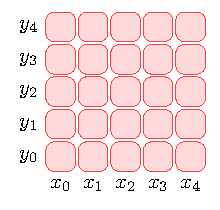
\includegraphics[height=0.4\textheight]{attnmask1.pdf}
      \end{minipage}
    }
    \subfigure[Left2Right Attention]{
      \begin{minipage}[b]{0.3\textwidth}
        \centering
        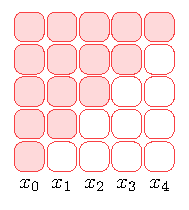
\includegraphics[height=0.4\textheight]{attnmask2.pdf}
      \end{minipage}
    }
    \subfigure[Mix Attention]{
      \begin{minipage}[b]{0.3\textwidth}
        \centering
        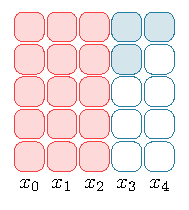
\includegraphics[height=0.4\textheight]{attnmask3.pdf}
      \end{minipage}
    }
  \end{figure}
}
\mframe{
  \frametitle{交叉注意力}
  \begin{columns}
    \begin{column}{0.5\linewidth}
      (Encoder-Decoder 模型)通过交叉注意力实现对 Encoder 表征的注意\\
      Corss Attention 中,$\mathbf{K}$ 和 $\mathbf{V}$ 来自 Encoder
    \end{column}
    \begin{column}{0.5\linewidth}
      \begin{figure}
        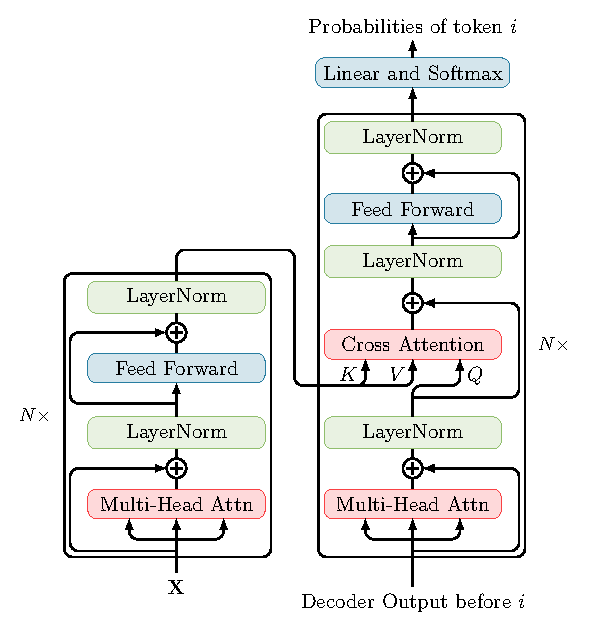
\includegraphics[height=0.8\textheight]{encoder-decoder.pdf}
      \end{figure}
    \end{column}
  \end{columns}
}
\mframe{
  \frametitle{一些噪声函数\Parencite{lewis2019}}
  \begin{itemize}
    \item Token Masking: 随机采样一些 tokens 并使用 [MASK] 替换
    \item Token Deletion: 随机删去一些 tokens,与 Token Masking 相比,这种方法迫使模型预测被删除的位置
    \item Text Infilling: 随机采样一些文本片段,并用遮罩 [MASK] 替换。这种噪声迫使模型预测被替换的文本片段的长度
    \item Sentence Permutation: 将文档按照句号分割成不同的句子,然后随机排列句子的顺序。这种噪声迫使模型学习同一文档中句子的顺序
    \item Document Rotation: 随机选择一个 token ,然后将文本旋转到以这个 token 为开头的状态。这种噪声训练模型识别文本开头的能力
  \end{itemize}
}
\begin{frame}[allowframebreaks]
  \frametitle{References}
  \printbibliography
\end{frame}
\mframe{
  \frametitle{BERT}
  BERT 的基本模型是一个双向 transformer 编码器,在经过大量文本数据的预训练之后,
  在 BERT 输出端添加 task head 并微调可以在下游任务上取得 sota 的结果,优于很多
  为任务特殊设计的模型结构。BERT 的出现使预训练-微调的模式成为 NLP 任务的事实标准

  BERT 的模型结构直接使用了 transformer\parencite{Vaswani2017a} 的 encoder 部分,
  作者在论文 \Citetitle{devlin2019} 中设计了两种大小的模型:
  $\text{BERT}_\text{BASE}(L=12,H=768,A=12,Total Parameters=110M)$和
  $\text{BERT}_\text{LARGE}(L=24,H=1024,A=16,Total Parameters=340M)$.
  其中,$L$ 是 transformer 层层数, $H$ 是模型隐藏维度,$A$ 是 multi-head attention 中的 head 数目
}
\mframe{
  \frametitle{BERT 的预训练-微调模式}
  \begin{figure}
    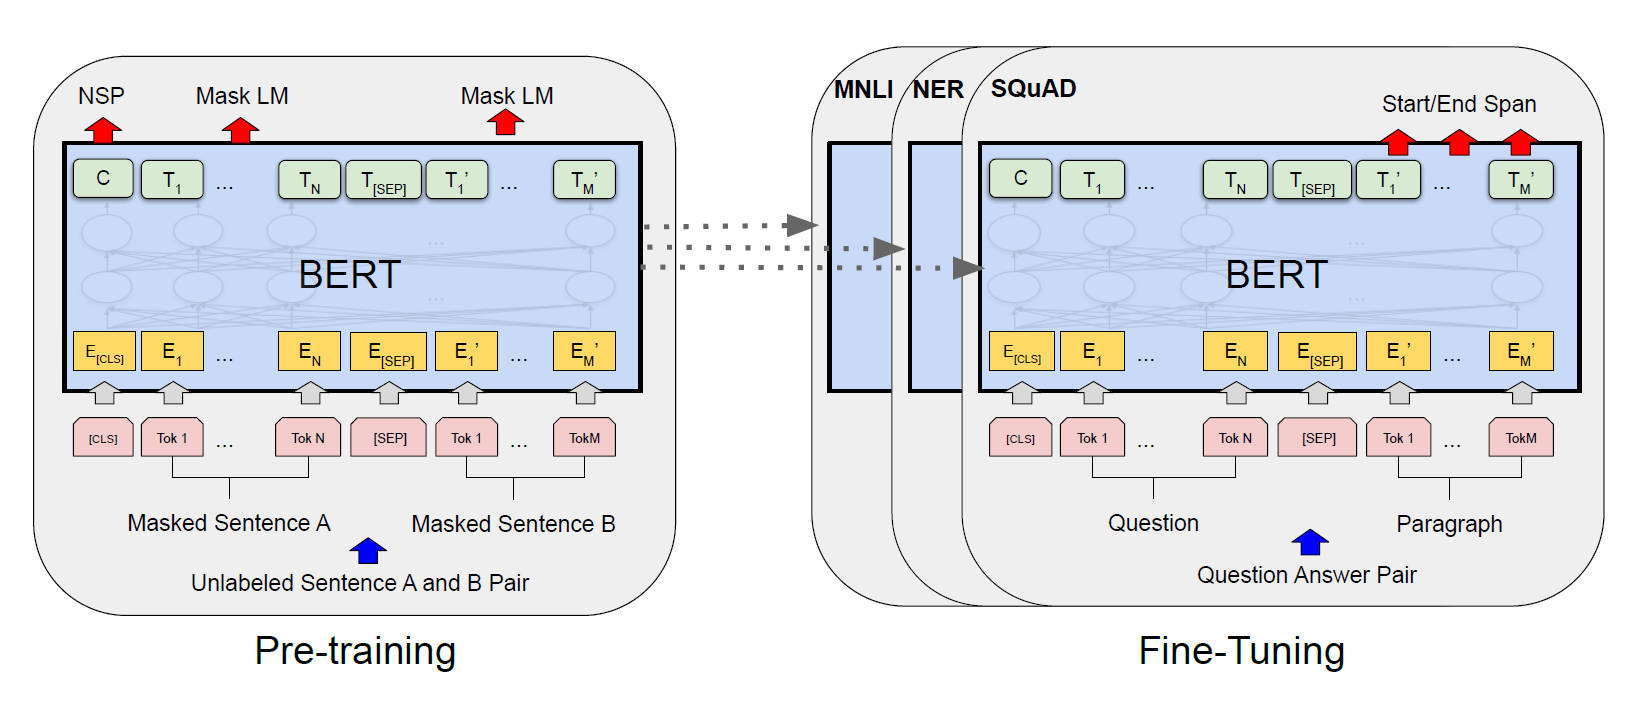
\includegraphics[width=\textwidth]{bert.png}
  \end{figure}
}
\newcounter{bert}
\stepcounter{bert}
\mframe{
  \frametitle{BERT 的 embedding 和输出表征 \Roman{bert}}
  BERT 的输入文本序列经过如下的处理后输入 embedding 层:
  \begin{itemize}
    \item 在整个序列头部添加特殊 token: [CLS]
    \item 在序列尾部以及句子的分隔处(在多句场景下)添加特殊 token: [SEP]
  \end{itemize}
  其中 [SEP] 指示句子的分割,这在部分多句任务中有用。[CLS] token 的表征将被用于
  句级分类任务,即 Sequence Classification 任务
}
\stepcounter{bert}
\mframe{
  \frametitle{BERT 的 embedding 和输出表征 \Roman{bert}}
    BERT 的 embedding 由三部分组成:
  \begin{figure}
    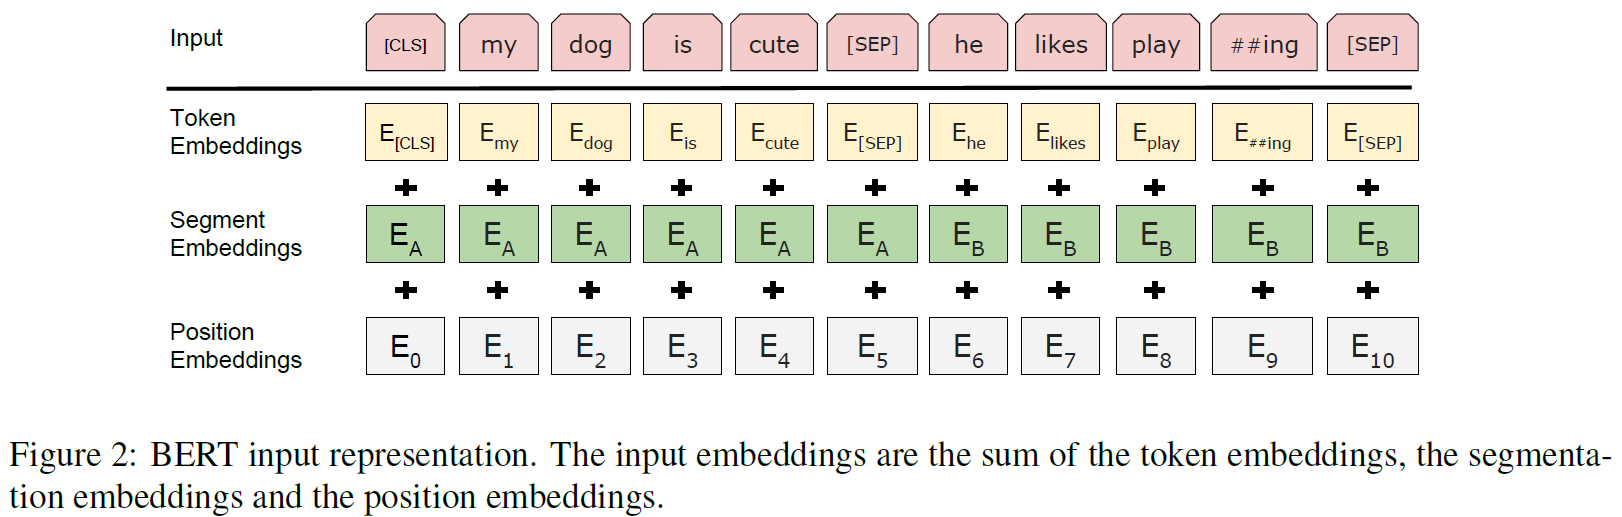
\includegraphics[width=\textwidth]{embedding.png}
  \end{figure}
  其中 segment embedding 指示该 token 属于输入文本中哪个句子(多句场景下),
  position embedding 指示该 token 在输入序列中的位置
}
\mframe{
  \frametitle{Pre-training}
  BERT 使用两个预训练任务:
  \begin{itemize}
    \item Masked Language Modeling(MLM): 在输入序列中随机抽取一部分 tokens,并替换为
    [MASK], 然后使用 BERT 去预测这些 tokens
    \item Next Sentence Prediction(NSP): 使用上文所说的 [CLS] token 进行序列分类,判断
    输入中的两个子句是不是原始文档中连续的句子
  \end{itemize}
  对于 MLM,其 [MASK] 的引入导致预训练和下游任务的割裂,BERT 使用下述策略弥补这种割裂:
  对于被选中的 tokens(15\%),并不总是将其替换为 [MASK], 而是:
  \begin{itemize}
    \item 80\% 替换为 [MASK]
    \item 10\% 保持不变
    \item 10\% 替换为字典中的随机词
  \end{itemize}
}
\mframe{
  \frametitle{fine-tuning}
  BERT 的预训练过程相当于为语言生成了较优的表征,在下游任务中使用 BERT 即使用这些表征。
  可以直接在 BERT 之后添加任务相关的层并端到端训练所有参数。
  例如,在分类任务中添加线性层和 softmax 函数
}
\mframe{
  \frametitle{The BERT Family}
  RoBERTa\Parencite{Liu2019} 在 BERT 的基础上使用更多的数据进行了更多的训练,同时研究了
  NSP 任务对性能的影响;
  XLNet\Parencite{Yang2019} 通过排序语言模型将 MLM 任务转化为 Autoregressive
  的形式,消除了 MLM 中的特殊 token: [MASK]; 
  SpanBERT\Parencite{Joshi2020} 在 BERT 的 MLM 基础上改进,使用 text span 粒度的 MASK 策略,提升 BERT
  的语言建模能力;
  ERINE\Parencite{Zhang2019a} 在 BERT 的基础上添加同样是 Transformer Encoder 结构的 Knowledge-Encoder,
  并使用 TransE\Parencite{Bordes2013} 作为嵌入层编码输入文本中的实体提及,在两种编码器之上使用知识融合层将实体
  表征融合到语言表征以实现语言表征中的实体知识注入;
  ERICA\Parencite{Qin2021} 关注于实体和关系的知识,在 BERT 的预训练
  过程中添加实体和关系相关的训练目标: Entity Discrimination, ED 和 Relation Discrimination, RD 实现了结构化
  知识向 PLM 的注入;
}
\end{document}
